\documentclass{article}
\usepackage{graphicx}
\usepackage{amsmath}
\usepackage{acronym}
\usepackage[backend=bibtex]{biblatex}

\title{Aposteriori Unimodality}
\author{Dimitris Tsirmpas, John Pavlopoulos}
\date{March 2025}


% Insert space after commas in math mode
\AtBeginDocument{%
  \mathchardef\stdcomma=\mathcode`,
  \mathcode`,="8000
}
\begingroup\lccode`~=`, \lowercase{\endgroup\def~}{\stdcomma\,}
\newcommand{\sdbdim}{\textit{dim}}
\newcommand{\Sdbdim}{\textit{Dims}}
\newcommand{\sdbgroup}{\textit{gr}}
\newcommand{\Sdbgroup}{\textit{Groups}}

\graphicspath{ {../graphs}  }
\bibliography{refs.bib}


\begin{document}

\maketitle

\section{Methodology}

In this section, we provide a formal mathematical formulation of the problem of attributing polarization to specific annotator characteristics (\S\ref{ssec:methodology:problem}), and offer an intuitive rationale for how established polarization metrics can be leveraged in this context (\S\ref{ssec:methodology:intuition}). We then introduce a comment-level measure that attributes polarization to individual \ac{SDB} factors (\S\ref{ssec:methodology:polstat}), and subsequently develop a statistical test that formalizes this attribution in a robust manner. Finally, we outline the technical details of the proposed methodology (\S\ref{ssec:methodology:details}).

\subsection{Problem Formulation}
\label{ssec:methodology:problem}

Let $d = \{c_1, c_2, \ldots\}$ be a discussion $d$ composed of $\lvert d \rvert$ comments.\footnote{Also referred to as “dialogue turns” in some publications.} We assume that annotating a comment depends on three variables: its contents, the annotator's \ac{SDB}, and uncontrolled factors such as mood and personal experiences. Assuming that each comment is assigned multiple annotators, we can define the annotation set $A(c)$ for comment $c$ as:
\begin{equation}
    A(c) = \{a(c, \theta) \mid \theta \in \Theta \}
\end{equation}
\noindent where  $a(c, \theta)$ is a single annotation for comment $c(d,i)$ and $\Theta$ is the set of annotator \acp{SDB}.

Since our goal is to pinpoint which specific characteristics contribute to polarization, we need a way to isolate individual attributes within a \ac{SDB}. $\Theta$ is usually composed of multiple ``dimensions'' (e.g., age, sex, educational level), each of which is composed of various groups. We can thus model $\theta \in \Theta$ as:

\begin{equation}
    \theta = \{(\sdbdim, \sdbgroup) \mid \sdbdim \in \Sdbdim, \sdbgroup \in \Sdbgroup(\sdbdim)\}
\end{equation} 
\noindent where $\Sdbdim =\{\sdbdim_1, \sdbdim_2, \ldots, \sdbdim_k\}$ is the set of \ac{SDB} dimensions, and $\Sdbgroup$ is the set of possible groups for dimension $\sdbdim$ (e.g., $\Sdbgroup(\sdbdim_{\textit{gender}}) = \{\textit{male}, \textit{female}, \ldots\}$).


\subsection{Quantifying changes in polarization}
\label{ssec:methodology:intuition}

Intuitively, dimension $\sdbdim$ partially explains polarization when the annotations divided according to each group $\sdbgroup \in \Sdbgroup(\sdbdim)$, show less polarization between each group compared to the full set of annotations. Figure~\ref{fig:ndfu_single_comment} exhibits a hypothetical example, where a misogynistic comment is annotated for toxicity by male and female annotators. The annotations are generally polarized ($nDFU_{all} = 0.625$), although the set of annotations from female annotators might exhibit low polarization between themselves ($nDFU_{women} = 0.100$---most agree the comment is toxic). The set of male annotations on the other hand, also shows low polarization ($nDFU_{men} = 0.3725$), but for the opposite reason---most men agree that it is \emph{not} toxic. This suggests that the overall polarization is driven by disagreements between male and female annotators. 

%TODO: Do I use 2 genders here?
%TODO: Use actual data in plot?
\begin{figure}
	\centering
	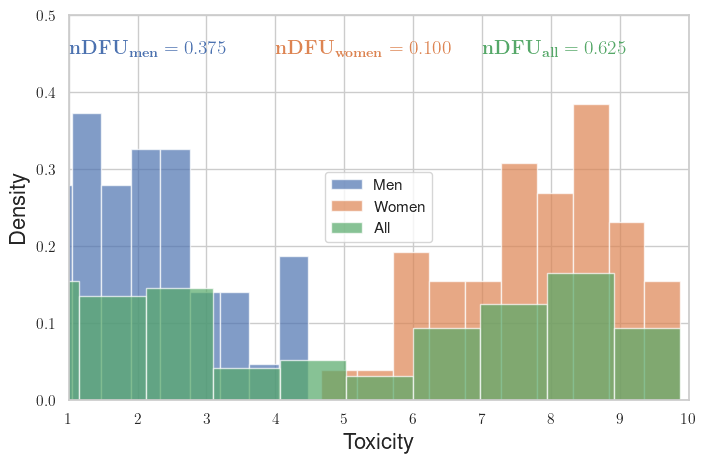
\includegraphics[width=0.8\linewidth]{ndfu_single_comment.png}
	\caption{Hypothetical example of a polarizing comment, where male and female annotators agree between themselves, but disagree with the opposite gender. Overall polarization ($nDFU_{all} = 0.625$) is much greater than the polarization exhibited by the annotations grouped by gender ($nDFU_{men} = 0.3725, nDFU_{women} = 0.100$). In this example, the annotation set $A$ was generated as $A_{men} \sim \mathcal{N}(2, 1.3), A_{women} \sim \mathcal{N}(8, 1.3), \lvert A_{men} \rvert = \lvert A_{women} \rvert = 50$.}
	\label{fig:ndfu_single_comment}
\end{figure}

Given this observation, we would be tempted to aggregate all annotations in a discussion. However, this formulation would not work well.  Figure~\ref{fig:ndfu_multi_comment} illustrates a hypothetical discussion with two comments, both of which are toxic, but where male and female annotators disagree on \emph{which} comment is the toxic one. If we aggregate the annotations for the two comments, the opposing polarization effects might balance each other out, leading to a false negative. In our example, while it is obvious that gender partly explains the polarization found in each of the individual comments ($nDFU_{all} \gg nDFU_{men}, nDFU_{all} \gg nDFU_{women}$), this observation is much harder to make when aggregating the two comments. To avoid this, we apply our statistic only on annotations that reference the same comment. 

\begin{figure}
	\centering
	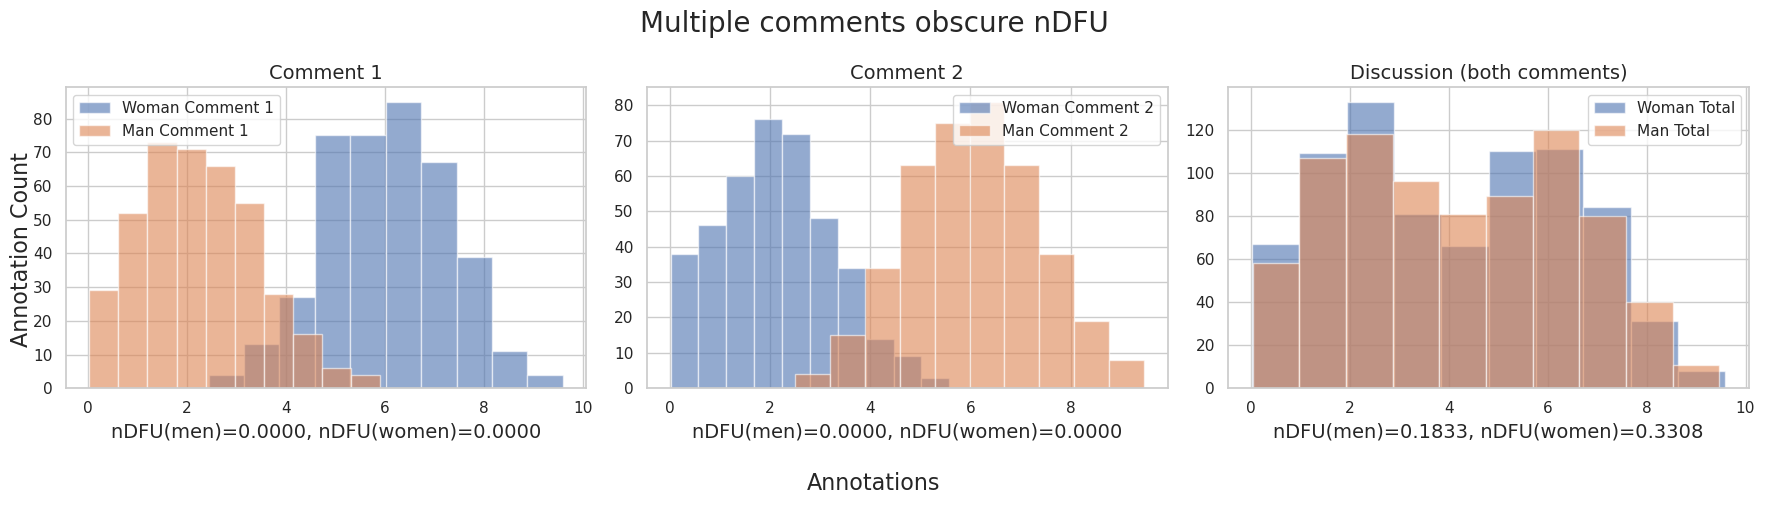
\includegraphics[width=\linewidth]{ndfu_multi_comments.png}
	\caption{Hypothetical example of a polarizing discussion with two comments, for which the annotators disagree which is the toxic one. If we aggregate the two comments, the polarization scores for both men and women significantly rise, obscuring whether the exhibited polarization can be partially attributed to gender. In this example, the annotation set $A$ was generated as $A_{men} \sim \mathcal{N}(6, 1), A_{women} \sim \mathcal{N}(2, 1), \lvert A_{men} \rvert = \lvert A_{women} \rvert = 200$ for the first comment, and $A_{men} \sim \mathcal{N}(2, 1), A_{women} \sim \mathcal{N}(6, 1), \lvert A_{men} \rvert = \lvert A_{women} \rvert = 200$ for the second.}
	\label{fig:ndfu_multi_comment}
\end{figure}

 
 
 \subsection{The pol-statistic}
 \label{ssec:methodology:polstat}
  
 The comment-level polarization statistic for group $\sdbgroup \in \sdbdim$ is obtained by:
 
 \begin{equation}
 	pol_{actual}(c, \sdbdim, \sdbgroup) = nDFU(P(A(c), \sdbdim, \sdbgroup))
 \end{equation}
 \noindent where $P(A(c),\sdbdim, \sdbgroup) = \{a(c, \theta) \in A | (\sdbdim, \sdbgroup) \in \theta\}$ is the partition of $A$ for a comment $c$, for which its annotators belong  to the group $\sdbgroup$ of \ac{SDB} dimension $\sdbdim$.
 
 If the polarization in a comment $c$ is driven by group $g$, we would expect polarization inside the groups to be higher than expected. We can estimate the expected polarization in comment $c$ between groups by randomly partitioning the comment's annotations in $\lvert \Sdbgroup(\sdbdim) \rvert$ groups, with each random group having size equal to that of the observed groups. For instance, if we have $100$ annotations, $80$ of which are made by male annotators and $20$ by female annotators, we will create random partitions of sizes $80$ and $20$. We can then sample the randomly partitioned annotations $t$ times. Formally the expected polarization will be given by:
 
 \begin{equation}
 	\label{eq:pol_expected}
 	pol_{expected}(c, \sdbdim, \sdbgroup) = \frac{1}{t} \sum_{i=1}^t  nDFU(\tilde{P}_i(A(c)))
 \end{equation}
 \noindent where each $\tilde{P}_i(A(c), \sdbdim, \sdbgroup)$ is a random partition of the annotation set $A(c)$ into $\lvert \Sdbgroup(\sdbdim) \rvert$ subsets with sizes matching the original, individual partitions ($\lvert \tilde{P}_i(A, \sdbdim, \sdbgroup) \rvert = \lvert P(A, \sdbdim, \sdbgroup) \rvert, \forall \sdbgroup \in \Sdbgroup(\sdbdim) , i=1, \ldots, t$).
 
 The difference between the observed and expected polarization for a comment $c$ given group $\sdbgroup \in \Sdbgroup(\sdbdim)$ is then given by the "pol-statistic", defined as: 
 
 \begin{equation}
	\textit{pol}(c, \sdbdim, \sdbgroup)  = pol_{actual}(c, \sdbdim, \sdbgroup)) - pol_{expected}(c, \sdbdim, \sdbgroup)
\end{equation}



\subsection{The Aposteriori Unimodality Test}
\label{ssec:methodology:aposteriori}

By obtaining the pol statistics for all comments in a discussion $d$ we can apply a mean test with the null hypothesis :

\begin{equation}
	\label{eq:null_h}
	H_0: \forall \sdbgroup \in \Sdbgroup(\sdbdim), \frac{1}{\lvert d \rvert} \sum\limits_{c \in d} pol(c, \sdbdim,  \sdbgroup) \le 0
\end{equation}
\noindent versus the (multiple) alternative hypotheses: 
\begin{equation}
	\label{eq:alt_h}
	H_{\sdbgroup}:\frac{1}{\lvert d \rvert} \sum\limits_{c \in d}  pol(c, \sdbdim, \sdbgroup) >  0
\end{equation}

We refer to this test as the \textit{``Aposteriori Unimodality Test''}, where a small p-value suggests that we can not rule out that annotators of the $\sdbgroup$ group make a significant contribution to the overall annotator polarization. The scope of the test and its relationship with the previously presented statistics are demonstrated in Figure~\ref{fig::overview}.

Our test assumes that there exist enough annotations in each comment and \ac{SDB} group to create a faithful histogram for \ac{nDFU} to effectively calculate polarization. Even in the presence of relatively few annotations however, assuming accurate \ac{nDFU} scores, the means test should provide a faithful estimate since we are aggregating annotations by comment.

\begin{figure}
	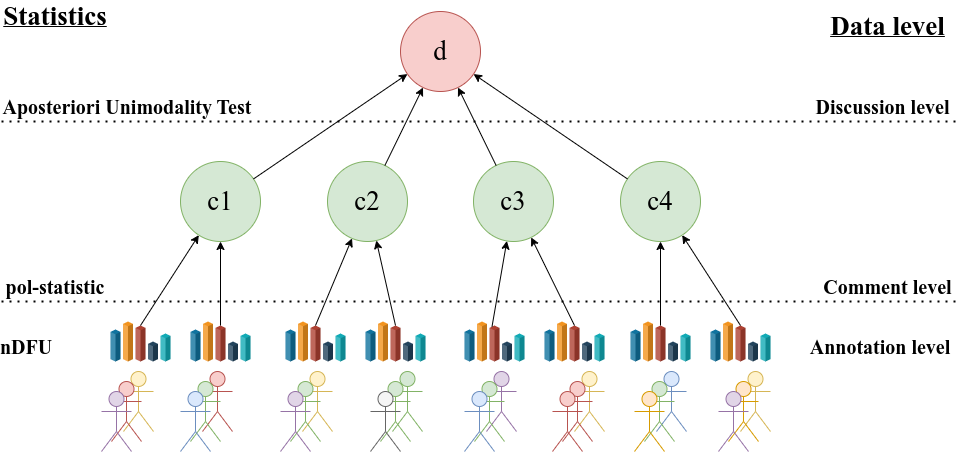
\includegraphics[width=\linewidth]{overview.png}
	\caption{An overview of the Aposteriori Unimodality Test. We gather statistical information from the annotations (different \acp{SDB} are denoted by different colors) via the \ac{nDFU} measure, which is aggregated on the comment-level by the pol-statistic. The Aposteriori Unimodality Test is applied on the discussion level, operating on the pol-statistics of the individual comments.}
	\label{fig::overview}
\end{figure}


\subsection{Technical Details}
\label{ssec:methodology:details}

The means test performed on the pol-statistics of each comment (Equations~\ref{eq:null_h},~\ref{eq:alt_h}) can be theoretically performed by most well-known statistical mean tests. In our case, we use the one one-sample Student t-test, since discussions are typically comprised of a moderately large amount of comments.

Additionally, since we are simultaneously considering $\lvert \Sdbgroup(\sdbdim) \rvert$ hypotheses, we apply a multiple comparison correction to the resulting p-values. We choose the Bonferroni method \parencite{Bland170}, since it is widely used, generally conservative, and especially so towards correlated hypotheses \parencite{ChenFengYi2017}. The last point is important, since many annotation groups are likely to be inter-correlated (e.g., age categories such as $50-60$ and $60-70$ years). Furthermore, one of its biggest weaknesses (the presence of very large numbers of hypotheses \parencite{ChenFengYi2017}) is unlikely to be met in annotation tasks.

Our test is actually parameterized by two more parameters: the $t$ parameter, which determines how many times we sample random partitions (Equation~\ref{eq:pol_expected}), and the \ac{FWER}, which is used to tune the strength of the multiple comparison correction mentioned above. We can increase the $t$ parameter to get a better estimate of the expected comment polarization, while increasing the computational cost of the method. We can also increase the \ac{FWER} to make our test more conservative towards multiple hypotheses \parencite{ChenFengYi2017}). In general, it is safe to set \ac{FWER} equal to the significance level of our test (e.g., $\textit{FWER} = 0.95$ if we are looking for $p < 0.05$)


\section{Acronyms}

\begin{acronym}[WWW]
    \acro{SDB}{SocioDemographic Background}
    \acro{nDFU}{normalized Distance From Unimodality}
	\acro{FWER}{Family-Wise Error Rate}
\end{acronym}

\printbibliography

\end{document}
